\title{QoS (Quality of Service) Improving Techniques}

\maketitle
\tableofcontents

%{{{

\section{Buffering (jitter hiding)}
%{{{

\begin{itemize}
\item Error-correction/congestion-avoiding techniques which are based
  on ARQ protocols sometimes produce a high jitter (variation of the
  latency).
\item Other times, the jitter is a direct consequence of the variation
  of the transmission bit-rates (most current transmission
  technologies use store-and-forward strategies and relatively large
  packets).
\item The simplest and most used technique to provide a seamless
  playback is by using a buffer at the receiver, which delays the
  reproduction of the stream a reasonable amount of time.
\item Example: YouTube.
\end{itemize}

%}}}

\section{Redundancy piggybacking}
%{{{

\begin{itemize}
\item Jitter (i.e., buffering time) can be minimized if some kind of
  information redundancy is introduced, avoiding the ARQ solution.
\item Example:
\end{itemize}
\begin{center}
  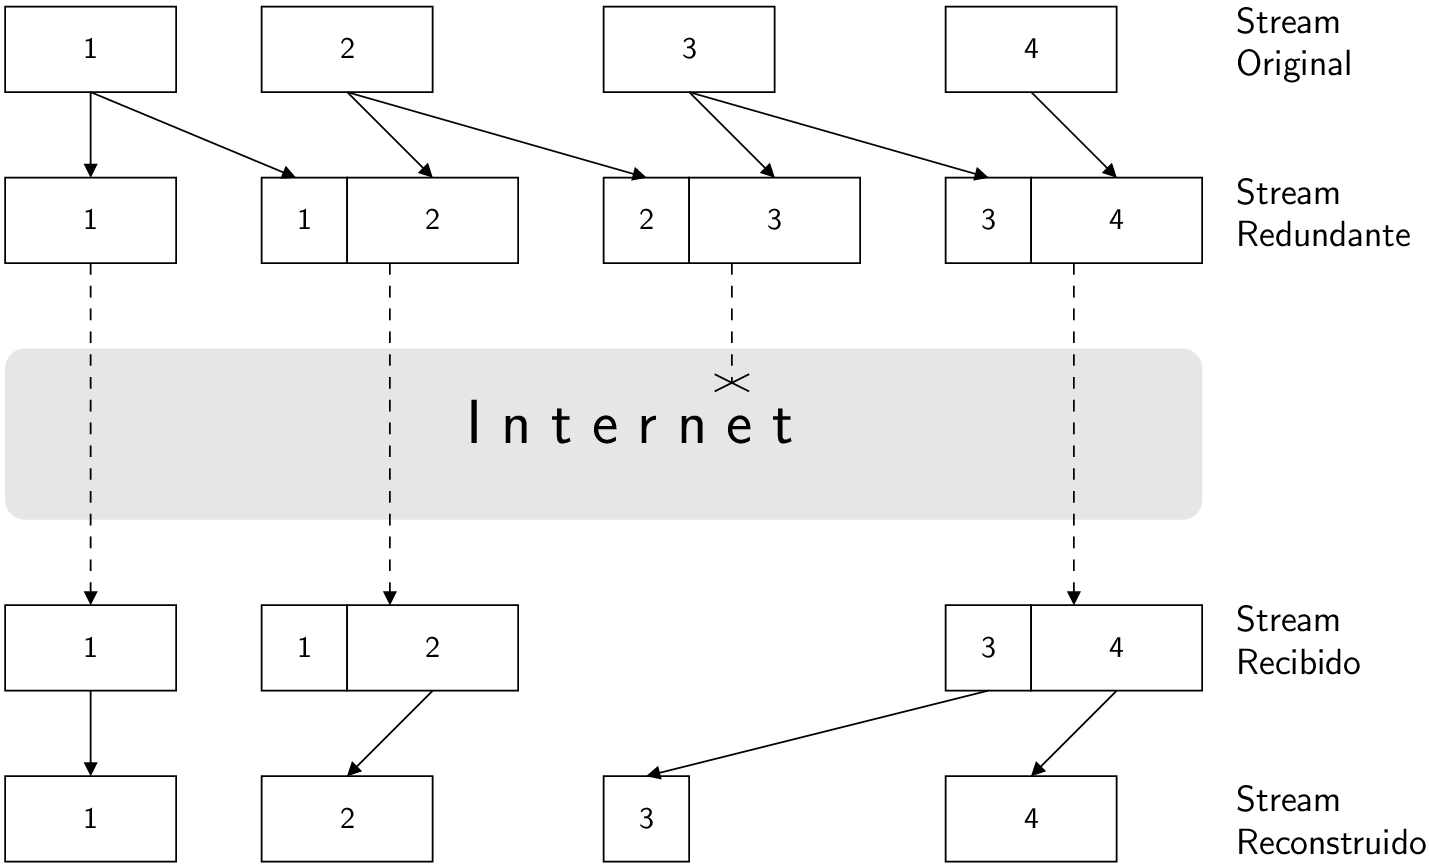
\includegraphics[width=\textwidth]{piggybacking}
\end{center}

%}}}

\section{Interpolation + Interleaving (increase quality in error-prone environments)}
%{{{

\begin{itemize}
\item Another technique for avoiding ARQ.
\item Most transmission errors produce a random alteration in a contiguous
  sequence of symbols (burst errors).
\item By interlaving the information before the transmission we spread
  the errors along the time (reducing the length of the bursts). Signal
  interpolation is easier if the burst errors are shorter.
\item Example:
\end{itemize}
\begin{center}
  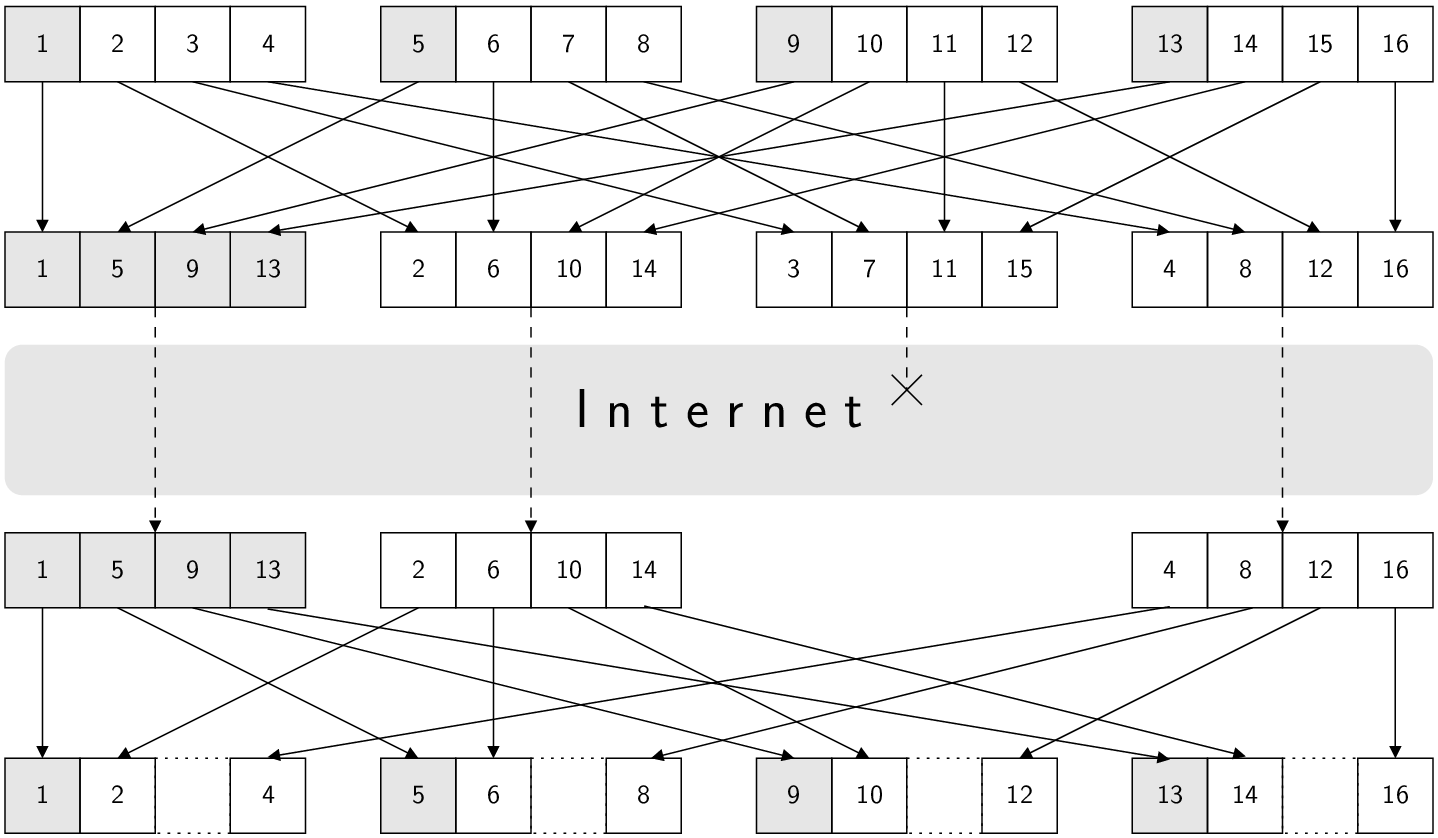
\includegraphics[width=\textwidth]{interleaving}
\end{center}

%}}}

\section{Buffer minimization}
%{{{

\begin{itemize}
\item Simulcasting and scalable video coding can help to minimize
  buffering times because receivers can modulate the bit-rate
  transmission of the senders.
\item In the case of using multiple description coding, the buffer
  will not underflow whenever at least one description is received.
\end{itemize}

%}}}

\section{Content-aware routing}
%{{{

\begin{itemize}
\item Multimedia traffic is time-sensitive.
\item Routers could prioritize multimedia data in order to minimize the
  latency and/or maximize the bit-rate of this information.
\item Unfortunately, this implies data-labeling and important changes
  in the current tarification system.
\end{itemize}

%}}}

%}}}
